\begin{frame}{How data is collected: HTTP request}
  \begin{figure}
    \centering
    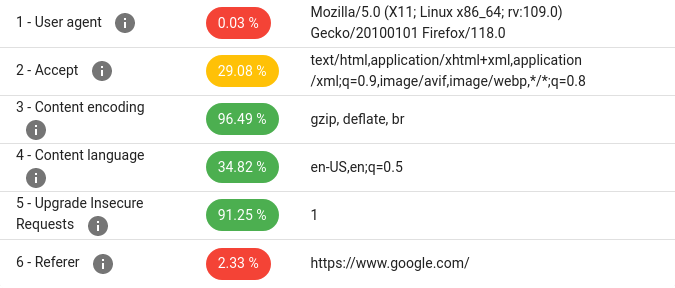
\includegraphics[width=\textwidth]{images/http-data.png}
  \end{figure}
\end{frame}

\begin{frame}{How data is collected: JavaScript attributes}
  \begin{figure}
    \centering
    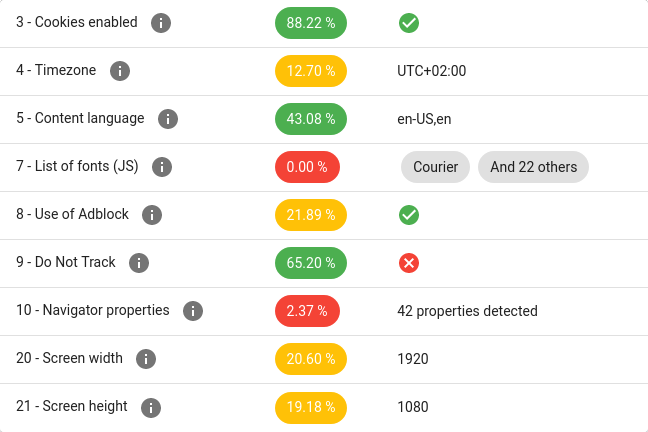
\includegraphics[width=\textwidth]{images/js-data.png}
  \end{figure}
\end{frame}

\begin{frame}{How data is collected: Canvas fingerprinting}
  The way an image or text is rendered on a canvas can vary based on the browser, os, gpu, font rendering settings and anti-aliasing algorithms, resulting in a unique image that can be used to create a fingerprint.
\end{frame}

\begin{frame}[fragile]{How data is collected: Canvas fingerprinting example}
  \begin{minted}{javascript}
// text with lowercase/uppercase/punctuation symbols
var txt = "BrowserLeaks,com <canvas> 1.0";
ctx.textBaseline = "top";
// the most common type
ctx.font = "14px 'Arial'";
ctx.textBaseline = "alphabetic";
ctx.fillStyle = "#f60";
ctx.fillRect(125,1,62,20);
// color mixing to increase the difference in rendering
ctx.fillStyle = "#069";
ctx.fillText(txt, 2, 15);
ctx.fillStyle = "rgba(102, 204, 0, 0.7)";
ctx.fillText(txt, 4, 17);
  \end{minted}

  \begin{figure}
    \centering
    \begin{subfigure}{0.45\textwidth}
      
\includegraphics[width=\linewidth]{images/canvas.png}
    \end{subfigure}
    \begin{subfigure}{0.45\textwidth}
      \animategraphics[loop, autoplay, width=\linewidth]{10}{images/frames/canvas}{00}{34}
    \end{subfigure}
  \end{figure}
\end{frame}

\begin{frame}{How data is collected: WebGL fingerprinting}

\end{frame}

\begin{frame}{How data is collected: TLS fingerprinting}

\end{frame}